\documentclass[preprint]{aastex}
\usepackage{epsfig}
\usepackage{color}
\usepackage{graphicx}
\usepackage{amssymb,amsmath}
\usepackage{natbib}

\definecolor{orange}{cmyk}{0,0.4,0.8,0.2}
\definecolor{darkorange}{rgb}{.71,0.21,0.01}
\definecolor{darkgreen}{rgb}{.12,.54,.11}
\definecolor{darkblue}{rgb}{0.1,0.1,0.8}
\definecolor{red}{rgb}{1.0,0,0}
\usepackage{hyperref}
\hypersetup{pdftex,  % needed for pdflatex
  breaklinks=true,  % so long urls are correctly broken across lines
  colorlinks=true,
  urlcolor=blue,
  linkcolor=darkorange,
  citecolor=darkgreen,
  }

\def\araa{{\it Ann.\ Rev.\ Astr.\ Ap.}}
\def\actaa{{\it Acta~Astronomica}}
\def\aj{{\it A.~J.}}  %Astronomical Journal%
\def\apj{{\it Ap.~J.}}  %Astrophysical Journal%
\def\apjs{{\it Ap.~J.~Suppl.}}  %Astrophysical Journal Supplements%
\def\apjl{{\it Ap.~J.~(Letters)}} %Astrophysical Journal Letters%
\def\pasa{{\it Pub.~A.S.A.}}  %Publications of the Astronomical Society of Australia
\def\pasp{{\it Pub.~A.S.P.}}      %Publications of the Astronomical%
                                %Society of the Pacific%
\def\memsai{{\it Memorie della Societ� Astronomica Italiana}}
\def\mn{{\it M.N.R.A.S.}}      %Monthly Notices of the Royal%
                                %Astronomical Society%
\def\mnras{{\it M.N.R.A.S.}}      %Monthly Notices of the Royal%
                                %Astronomical Society%
\def\nat{{\it Nature}}      %Nature%
\def\aa{{\it Astr.~Ap.}}     %Astronomy & Astrophysics%
\def\aap{{\it Astr.~Ap.}}     %Astronomy & Astrophysics%
\def\aasup{{\it Astr.~Ap.~Suppl.}}     %A & A Supplements%
\def\aaps{{\it Astr.~Ap.~Suppl.}}     %A & A Supplements%
\def\ass{{\it Astr.~Sp.~Sci.}}     %A & A Supplements%
\def\ssr{{\it Space Sci. Rev.}}   %Space Science Reviews%
\def\an{Astronomische~Nachrichten}%

\def\sdss{SDSS}
\def\wise{WISE}
\def\allwise{ALLWISE}
\def\twomass{2MASS}
\def\ogle{OGLE-III}
\def\macho{MACHO}
\def\simbad{SIMBAD}
\def\mw{Milky Way}
\def\agb{AGB}

\begin{document}
\title{The Three-Dimensional Distribution of Galactic AGB Stars with ALLWISE}
\shorttitle{The 3D Distribution of Galactic ALLWISE AGB Stars}
\author{Nicholas M. Hunt-Walker, \v{Z}eljko Ivezi\'{c}, Andrew C. Becker}
\affil{University of Washington, Department of Astronomy, Seattle, WA 98195}
\email{nmhw@uw.edu, ivezic@uw.edu, acbecker@uw.edu}
\shortauthors{Hunt-Walker, Ivezi\'{c}, \& Becker}
\maketitle

% Abstract
\begin{abstract}
We study the structure of the Milky Way disk with candidate asymptotic giant branch (AGB) stars selected from the \emph{Wide-field Infrared Survey Explorer} (\emph{WISE}) catalog. The advantages of our approach, compared to most recent similar works such as those based on SDSS data, are large distance limits due to the high luminosity of AGB stars, small interstellar dust obscuration due to longer wavelengths, and the all-sky coverage of the \emph{WISE} survey. The candidate AGB stars are color-selected with high completeness and low contamination, as quantified using samples of known AGB stars and other objects with known classifications from the SIMBAD and \emph{Sloan Digital Sky Survey} (\emph{SDSS}) databases. Distances to candidate AGB stars are estimated simultaneously with interstellar dust extinction along the line of sight using a 3-dimensional dust distribution model developed to support simulations for the \emph{Large Synoptic Survey Telescope} (\emph{LSST}) and a color -- absolute magnitude relation calibrated using the Large Magellanic Cloud (LMC) and the Galactic bulge. We find that the Galactic disk extends radially out to 15 kpc, with flaring of the disk towards its edge. We present measurements of the vertical scale height and horizontal scale length for double-exponential disk models. We find that the density distribution of AGB candidates within 9 kpc from the Galactic center is consistent with that of a double-exponential profile, while at larger radii the distribution is indistinguishable from a single-exponential profile.
\end{abstract}


% Introduction
Nick was here
\section{Introduction}
%The formation of galaxies like the \mw\, was long thought to be a steady process that created a smooth distribution of stars. This standard view was exemplified by the \cite{1980ApJS...44...73B} and \cite{1989ARA&A..27..555G} models, described in detail by, e.g., \cite{1993ARA&A..31..575M}. It was further motivated by observations of other galaxies, as well as what little information was available from \emph{High Precision Parallax Collecting Satellite} \citep[\emph{HIPPARCOS}, ][]{1984SSRv...39....1K} and smaller pencil-beam surveys. In these, 
The structure of the \mw\, has for many years been uncertain, with historical models assuming three discrete components described by simple analytic expressions: the thin disk, thick disk, and halo \citep{1980ApJS...44...73B, 1989ARA&A..27..555G,1993ARA&A..31..575M}. 
The advent of the \emph{Sloan Digital Sky Survey} \citep[\sdss, ][]{2000AJ....120.1579Y} has since provided more detail, using accurate digital multi-band optical photometry across a quarter of the sky, as well as the largest optical spectroscopic catalog thus far known. 
%This new influx of data enabled the development and application of photometric parallax methods, using color-magnitude relations to estimate stellar distances.
These new data led to the large scale ``tomography" of the \mw\; via stellar distributions in the 7-dimensional space spanned by spatial coordinates \citep{2008ApJ...673..864J}, velocity components \citep{2010ApJ...716....1B}, and metallicity \citep{2008ApJ...684..287I}. The resulting maps revealed rich, complex substructure in the distribution of the \mw's stars \citep[e.g.][]{2000AJ....120..963I,2000ApJ...540..825Y,2001ApJ...554L..33V,2002ApJ...569..245N,2003ApJ...599.1082M,2006ApJ...642L.137B,2006ApJ...651L..29G,2006AJ....132..714V}, deeply shaking the existing view of the Galaxy. 

In order to move forward from where \sdss\, tomography left off, we require observations that span an area larger than that of \sdss\,, with Galactic objects that can be seen through interstellar dust out to large distances. Stars from the Asymptotic Giant Branch (\agb) are perfect candidates to serve as these probes to the \mw. \agb\, stars represent the last stage of evolution for stars between 0.8 and 8 $M_\odot$ \citep{1983ARA&A..21..271I, 2005ARA&A..43..435H} -- the mass-range with the highest number of stars as inferred from the  \cite{2001MNRAS.322..231K} initial mass function that can also reach the final stages of stellar evolution within a galactic timescale. Because of this, they are bound to reside throughout the galaxy wherever other stars are present. This phase of evolution is marked by two distinct periods: the early \agb\, (E-\agb)  and the thermally-pulsing \agb\, phases. During the latter of the two, \agb\, stars produce substantial dust-driven stellar winds \citep[$10^{-7} < \dot{M} < 10^{-4}$ $M_\odot$ yr$^{-1}$,][]{2002A&A...391.1053O} rich in oxides (SiO, Al$_2$O$_3$, etc.) and carbon-rich molecules (SiC, AmC, etc.), with the chemical dominance being highly dependent upon the metallicity of the host galaxy \citep{2005A&A...434..691M}. Galaxies such as the Milky Way are expected to have a substantial population of oxygen-rich AGB stars \citep{1985A&A...152L...1H}, whereas low-metallicity galaxies such as the Magellanic clouds have been shown to possess AGB populations dominated by carbon-rich stars \citep{2011AJ....142..103B}. In both cases, the other species of AGB star is rarely seen, as richness in one chemical type (e.g. oxides)  necessitates the almost complete capture of the other chemical type (e.g. carbon) in CO \citep{1983ARA&A..21..271I}. Over time, these chemically-rich winds create vast circumstellar shells that, when warmed by the stellar photosphere, emit in the near- and mid-infrared (NIR \& MIR respectively). Although the molecular species present in oxygen- and carbon-rich winds are vastly different, emission from both types produce strong IR emission near 10$\mu$m, visible out to the Magellanic clouds \citep{2011A&A...534A..79I} and beyond. Thus, if these stars can be pinpointed by a survey with a wide area of observation and high positional accuracy, they can be used as markers for a map of the Milky Way \citep{2013RAA....13..323T}.

Such a survey can be found in the \emph{Wide-field Infrared Survey Explorer} \citep[\wise, ][]{2010AJ....140.1868W, 2012wise.rept....1C}, a space-based observatory that has imaged the entire sky in the MIR (3.4, 4.6, 12, and 22$\mu$m). Additionally, \wise\, has been positionally matched to the Two-Micron All-Sky Survey (\twomass), a four-year mission characterizing the full sky in the NIR. Thus, the \wise\, catalog presents with hundreds of millions of sources with photometry of unprecedented sensitivity and positional accuracy in the NIR and MIR--ideal for capturing \agb\, stars at Galactic distances. In this paper, we use samples of known Galactic and Magellanic \agb\, stars to formulate color-color criteria with \wise\, and \twomass\, photometry that can produce a reliable catalog of IR \agb\, candidates. We then use these candidates in conjunction with estimates of Galactic dust extinction along the line of sight to produce a Galaxy-wide number density distribution of \agb\, stars.  

In Section~\ref{sec:data}, we describe in detail the data that we use for our study. In Section~\ref{sec:criteria}, we describe the color-color criteria used to isolate \agb\, stars in the \wise\, dataset, and the color-magnitude relationships that were derived for these stars from the Large Magellanic Cloud and the \mw\, bulge.
In Section~\ref{sec:distribution}, we describe the spatial density distribution of \agb\, candidates in the Milky Way.
Our conclusions can be found in section~\ref{sec:conclusions}.


% Data Sources and Reduction
\section{Data Sources and Reduction}
\label{sec:data}


\subsection{Data Sources}
\label{sec:sources}
In this study, we rely heavily on data from the \allwise\, extension of the \wise\, survey, combining data from the initial All-Sky Data Release, the 3-band cryogenic data release, and the NEOWISE post-cryogenic data release \citep{2013wise.rept....1C}. The initial \wise\,All-Sky Data Release observed the sky between January and August 2010, observing the sky 1.2 times with four detectors, operating at 3.4, 4.6, 12, and 22$\mu$m. Hereon we refer to \allwise\, photometric bands at [3.4$\mu$m/4.6$\mu$m/12$\mu$m/22$\mu$m] as [$W1/W2/W3/W4$]. The positions of objects in the \wise\, catalog were calibrated to the \twomass\, point source catalog. The 3-band cryogenic data release contains data from $W1$, 2, and 3, and surveyed $30\%$ of the sky between August and October 2010. During the 3-band cryogenic survey, $W1$ and $W2$ operated with nearly the same sensitivity as during the full survey. Warming of the telescope reduced sensitivity in $W3$ and fully saturated $W4$. The NEOWISE post-cryogenic data release contains $W1$ and $W2$ measurements, with sensitivities close to those obtained during the full cryogenic phase. During this phase, \wise\, surveyed $70\%$ of the sky. Data products from the post-cryogenic release included updated instrumental, astrometric, and photometric calibrations and reduction algorithms, resulting in much lower SNR. The overall number of sources compiled into \allwise\, totals over 747.6 million.

In order to generate a reliable, high-confidence catalog of Galactic candidate \agb\, stars, we must first define color-color criteria from known \agb\, star samples. We select \agb\, stars from three source catalogs: the {\it Optical Gravitational Lens Experiment-III Variable Star Catalog} \citep[\ogle,][]{2008AcA....58...69U,2009AcA....59..239S,2011AcA....61..217S}, the {\it MAssive Compact Halo Objects} project \citep[\macho,][]{1997ApJ...482...89A}, and the \simbad\, Astronomical Database \citep{2000A&AS..143....9W}. 

\ogle\, photometry for Long-Period Variables (LPVs) in the Small and Large Magellanic Clouds (SMC and LMC respsectively) was obtained between July 2001 and May 2009, with stars in the central 4.5-deg$^2$ of the LMC and SMC having an additional 5 observing seasons of photometry from OGLE-II. LPVs were classified into 3 categories: \ogle\, Small Amplitude Red Giants (OSARGs), Semi-Regular Variables (SRVs), and Miras. All AGB stars  O-rich and C-rich \agb\, stars in \ogle\, were photometrically selected using reddening-free Wesenheit magnitudes, described in detail in \cite{2009AcA....59..239S,2011AcA....61..217S}. {\color{red}[Describe the selection bit in a little more detail, along with their sample completeness, selection biases, and contamination fractions]} Data reduction techniques are described in \cite{2008AcA....58...69U}. The resulting samples yield 46,467 \agb\, stars from the LMC (37,203 O-rich; 9,264 C-rich) and 6,509 stars from the SMC (3,727 O-rich; 2,782 C-rich). 

From \macho\, we obtain the sample of SMC, LMC, and Galactic Bulge AGB stars used in \cite{2008AJ....136.1242F} (14,861 stars). {\color{red}Why were these objects selected? Howe were they selected? What is their completeness, selection bias, and contamination fraction?} Following \cite{2008AJ....136.1242F}, the objects are divided into sequences (seq) 1-4. Sequence 1 primarily contains Mira variables pulsating in their fundamental modes, whereas Sequences 2-4 contain semi-regular variables in various pulsation modes.

The sample of AGB stars from \simbad\, was obtained by querying all objects classified as C-stars (18,656), S-stars (1,108), OH/IR stars (825), AGB stars (2,359), and Mira variables (9,608), for a total of 32,556 stars. Objects are classified spectroscopically, though by a variety of methods owing to the heterogeneous data housed within \simbad. Together with \macho\, and \ogle, the total sample of \agb\, stars is 100,393. Because there is a high likelihood that samples between \ogle, \macho, and \simbad overlap, we retain only unique objects after the initial data reduction in section~\ref{sec:reduction}.

We use \sdss\, spectroscopic catalogs to find and quantify regions in NIR-MIR color-color space populated by plausible contaminant sources. These include any Galactic stellar objects and planetary nebulae, as well as a host of extragalactic sources. Data for active galactic nuclei (AGN; 19,184 objects), quasi-stellar objects (QSOs; 122,550 objects), and star forming/burst galaxies (820,272 objects total) were drawn from \sdss\, DR7, specifically from the NYU Value Added Galaxy Catalog\footnote{\url{http://sdss.physics.nyu.edu/vagc/}} \citep[VAGC]{2005AJ....129.2562B}. Luminous Red Galaxies (LRGs) were selected from the SDSS Luminous Red Galaxy Survey \citep[105,631 objects, ][]{2010ApJ...710.1444K}.  Data for stars in the SDSS stellar locus were drawn from the DR 9 SEGUE Stellar Parameters Pipeline (SSPP) \citep[1,843,190 objects, ][]{2012ApJS..203...21A}. {\color{red} Include bit about YSOs and PNe from SIMBAD}

\subsection{Data Reduction}
\label{sec:reduction}
We use NASA/IPAC IRSA's {\tt GATOR} tool\footnote{\url{http://irsa.ipac.caltech.edu/cgi-bin/Gator/nph-scan?mission=irsa&submit=Select&projshort=WISE}} to positionally match \sdss, \ogle, \macho, and \simbad\, to \allwise. We select only matches within 3" between  each sample and \allwise. All samples of \agb\, were required to be brighter than the published 5$\sigma$ faint limits of [16.83/15.6/11.32/8.0], as well as fainter than the saturation limits of [2.0/1.5/-3.0/-4.0] extrapolated from the wings of the PSFs for point sources, for [$W1/W2/W3/W4$] \citep{2013wise.rept....1C}, with no flags for confusion or contamination as a spurious source in any band. We also require only single associations with \twomass\, objects within 3", detections in [$J/K_S/W1/W2/W3/W4$], and SNR $>$ 3 in each \allwise\, band. 

The population for each sample from initial matching as well as after the application of the \allwise\, faint limits, saturation limits, and \twomass\, detection requirements are shown in Table~\ref{tab:pop}. The WISE color-color distributions for the AGB and contaminant samples are shown in Figure~\ref{fig:distros}. \\

\vspace{-10pt}
%\begin{table}[h]
%	\begin{center}
%	\caption{AGB and Contaminant Populations}
%	\scalebox{0.85}{\begin{tabular}{l c c c c c c}
%		\hline
%		Population & SIMBAD C stars & OH/IR stars & Miras & S stars & AGB stars \\
%		\hline
%		2" match & 13,245 & 294 & 8,850 & 1,078 & 1,665 \\
%		Reduced & 3,327 & 165 & 6,218 & 865 & 1,121 \\
%		\hline\hline
%		Population & MACHO seq1 & seq2 & seq3 & seq4\\
%		\hline
%		2" match & 5,193 & 3,441 & 2,548 & 2,931 \\
%		Reduced & 927 & 642 & 263 & 336 \\
%		\hline\hline
%		Population & OGLE C-rich & O-rich\\
%		\hline
%		2" match & 11,417 & 38,369 \\
%		Reduced & 737 & 2515 \\
%		\hline\hline
%		Population & Locus Stars & AGN & LRG & QSO & Galaxies \\
%		\hline
%		2" match & 1,508,158 & 18,481 & 102,178 &  & 799,761 \\
%		Reduced & 168,045 & 9,652 & 7,717 & 18,360 & 125,869 \\
%		\hline
%
%		\label{tab:pop}
%	\end{tabular}}
%	\end{center}
%\end{table}

\begin{table}[h]
	\begin{center}
	
	\scalebox{0.85}{\begin{tabular}{l c c c c c c}
		\hline\hline
		Population & SIMBAD AGB* & C* & Mira & OH/IR & S* \\ 
		\hline
		3" match & 1,689 & 14,209 & 9,027 & 406 & 1,081 \\
		Reduced & 684 & 1,782 & 3,241 & 43 & 511 \\ 
		\hline
		Population & MACHO seq1 & seq2 & seq3 & seq4 \\ 
		\hline
		3" match & 5,279 & 3,519 & 2,619 & 3,070 \\
		Reduced & 277 & 185 & 73 & 61 \\ 
		\hline
		Population & OGLE-III C-rich & O-rich \\ 
		\hline
		3" match & 11,542 & 38,848 \\
		Reduced & 249 & 730 \\ 
		\hline
		Population & DR12 SSPP & DR7 LRG & QSO & AGN & Galaxies \\ 
		\hline
		3" match & 1,578,329 & 104,345 & 103,590 & 18,528 & 841,712 \\ 
		Reduced & 67,508 & 84 & 3,977 & 1,069 & 44,314 \\ 
		\hline\hline

		
	\end{tabular}}    
	\caption{\agb\, and contaminant populations matched to WISE before and after sample reduction in section~\ref{sec:reduction}. MACHO sequences (seq1-seq4) are from \cite{2008AJ....136.1242F} and described briefly in section~\ref{sec:sources}.\label{tab:pop}}
	\end{center}
	
\end{table}

\begin{figure}
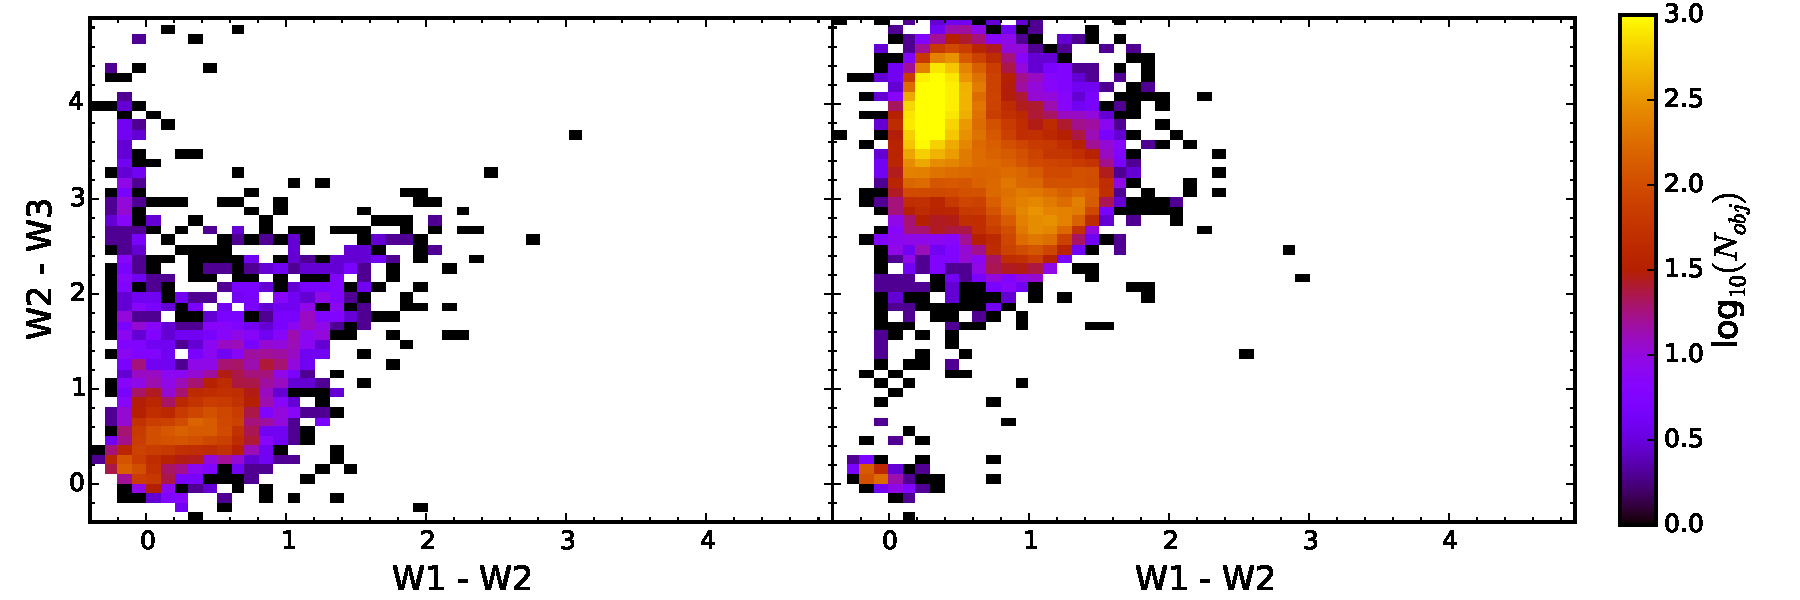
\includegraphics[width=7in]{figs/agbs_contaminants_color_color1.pdf}
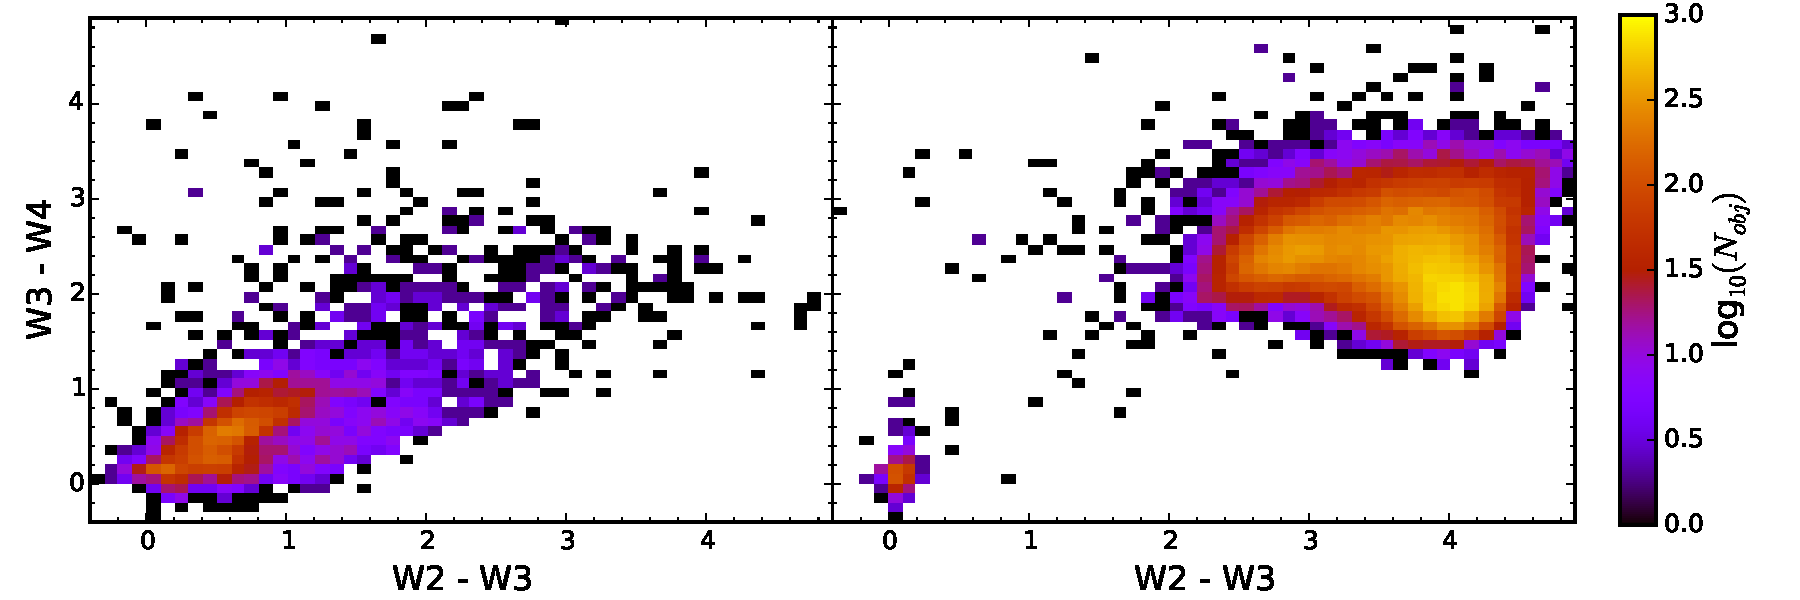
\includegraphics[width=7in]{figs/agbs_contaminants_color_color2.pdf}
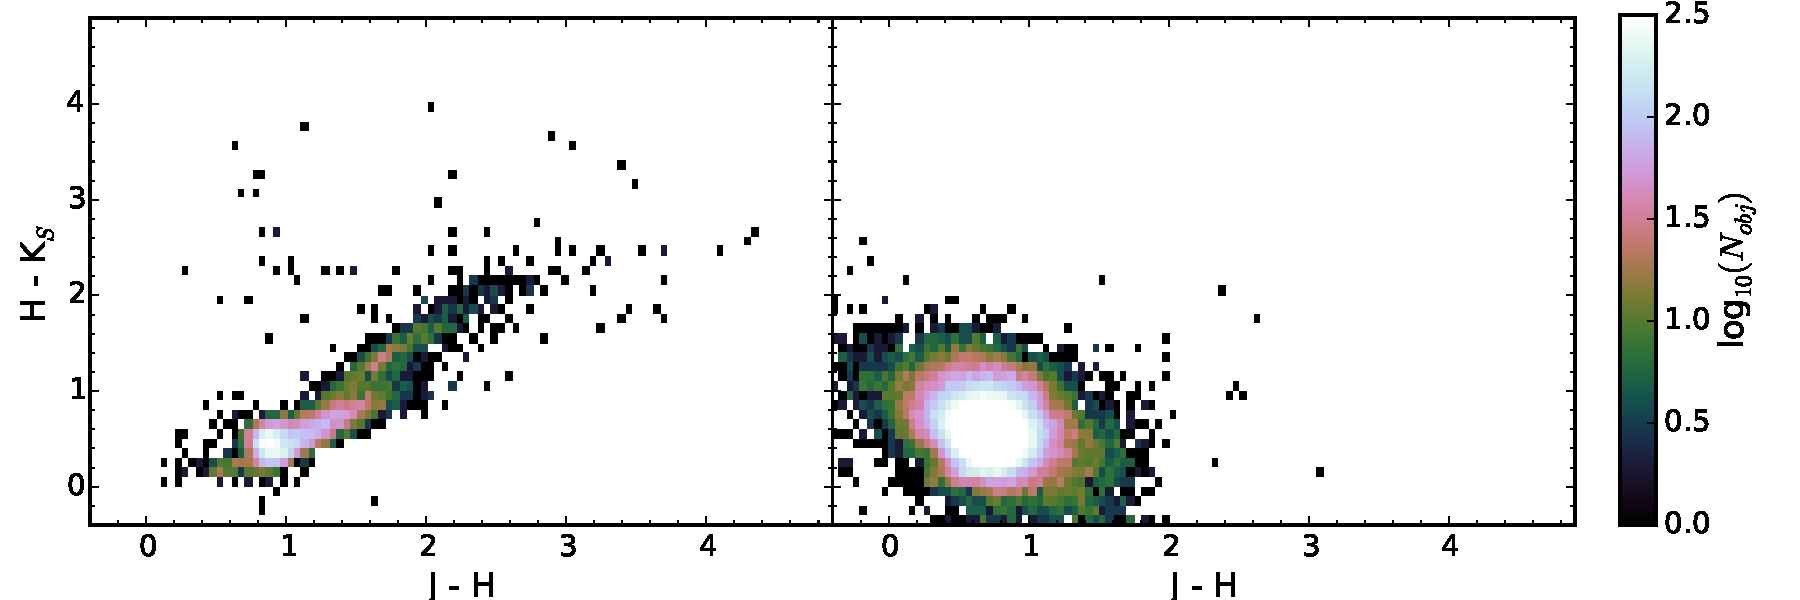
\includegraphics[width=7in]{figs/agbs_contaminants_color_color3.pdf}
\caption{Logarithmic number densities for objects in \wise\, and \twomass\, color-color space, binned in 0.1 dex on each axis. \emph{Left:} The combined AGB sample matched to ALLWISE. \emph{Right:} The combined contaminant sample.\label{fig:distros}}
\end{figure}



% Selection
\section{Object Selection Criteria}
\label{sec:criteria}
We create color-color criteria to generate a catalog of AGB candidates. We seek to maximize AGB completeness while minimizing contamination from non-AGB objects to beneath the 1\% level.

The color-color criteria for AGB selection are as follows:
\begin{align} 
(J-K_s) > 1.1\label{eq:criteria1}\\
(W2-W3) > 0.3\label{eq:criteria2}\\
(W3-W4) < -0.83(W2-W3) + 3.37\label{eq:criteria3}
\end{align}
The criteria in (1) and (2) are primarily concerned with rejecting objects from the stellar locus, and other stars whose NIR spectra are dominated by the Rayleigh-Jeans tail (many covered by the sample of galaxies).  Criteria in (3) also reject stars from the stellar locus, but primarily function to reject IR-bright extragalactic sources.

\noindent Sample completeness $\eta$ is defined as
\begin{eqnarray*}
\eta &=& \frac{N - n_\text{missed}}{N}
\end{eqnarray*}
where $N$ is the total number of objects in that sample, and $n_\text{missed}$ is the number of objects outside of the applied boundaries. Figure~\ref{fig:completeness} shows the distribution of completeness amongst AGB sources after the application of the above criteria. Sample contamination is typically defined as
\begin{eqnarray*}
\epsilon &=& \frac{n_\text{spurious}}{n_\text{selected}}.
\end{eqnarray*}
where $n_\text{spurious}$ is the number of spurious sources and $n_\text{selected}$ is the total number of selected sources, including AGB objects and spurious objects \citep{2013sdmm.book.....I}. The contamination map is shown in Figure~\ref{fig:contamination}.

\begin{figure}[h]
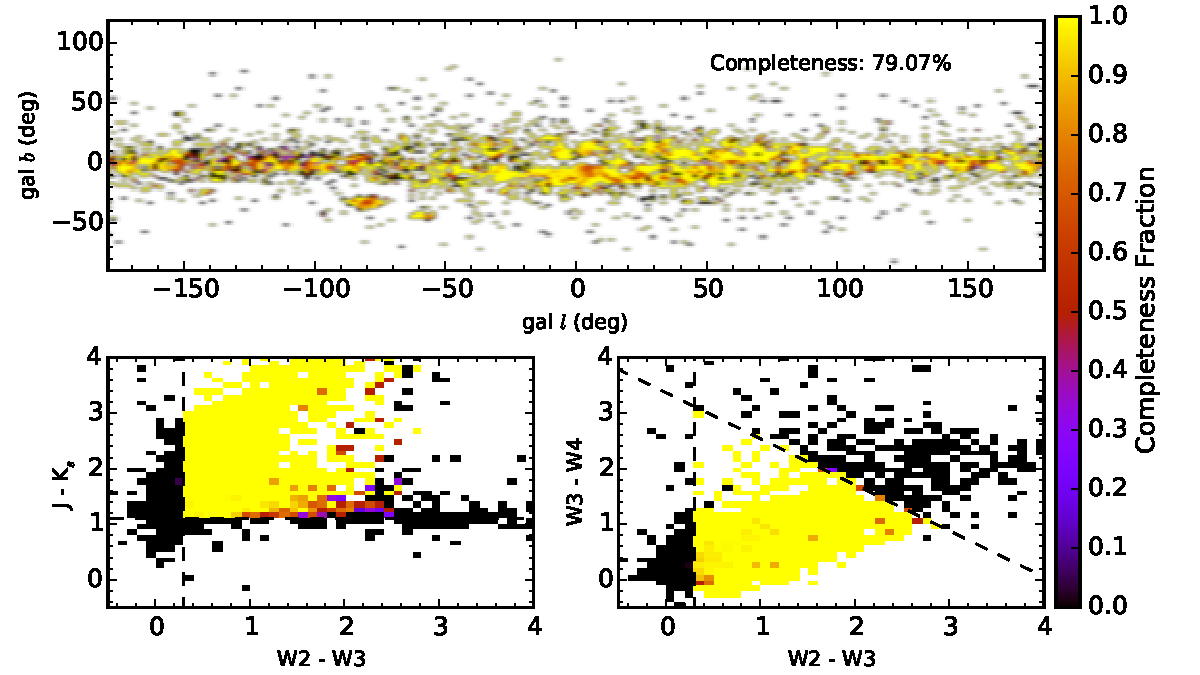
\includegraphics[width=6.7in]{figs/completeness_map.pdf}
\caption{Words \label{fig:completeness}.}
\end{figure}
\begin{figure}[h]
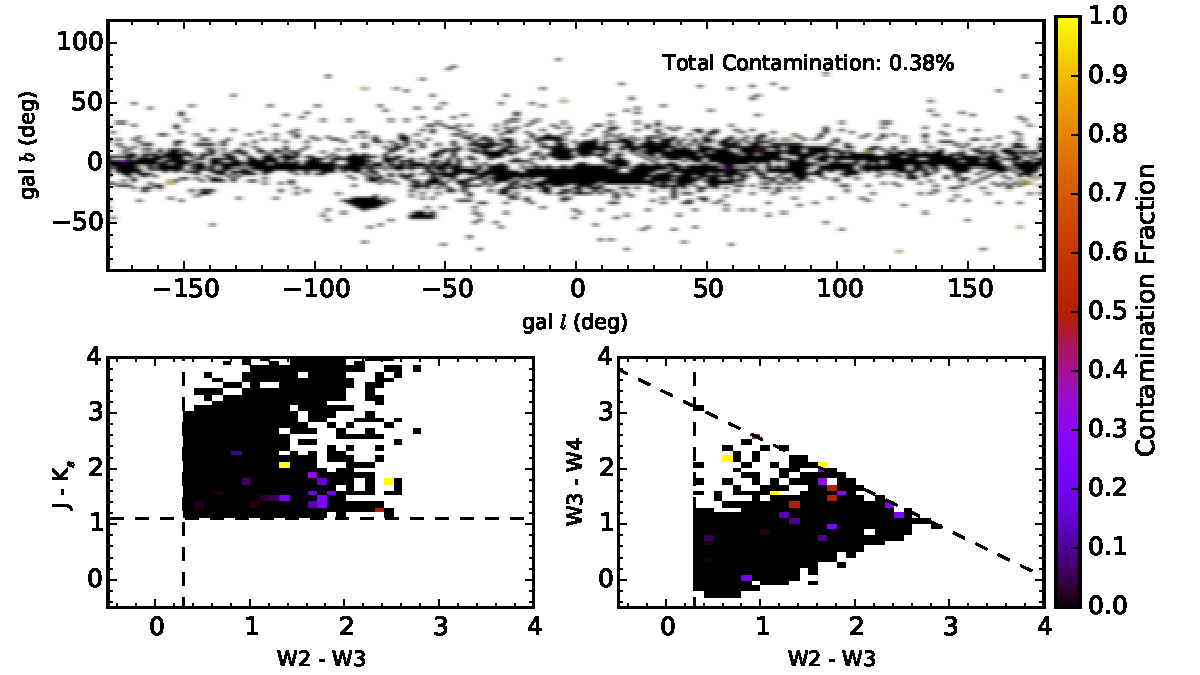
\includegraphics[width=6.7in]{figs/contamination_map.pdf}
\caption{Words \label{fig:contamination}.}
\end{figure}

A fairly large issue for creating the boundaries are the O-rich stars.  Either the objects from the OGLE O-rich AGB star catalog were mostly mis-matched to WISE, taking on colors of the stellar locus, or the issue is more physical.  It could be that the warm O-rich AGB photospheres are still visible and not heavily enshrouded in dust, thus appearing similar to Main Sequence stars in the NIR. Previous work on warm O-rich AGB stars has shown that their circumstellar shells are not prominent, and their NIR photometry reflects the Rayleigh Jeans tail of a cool 2000-4000K blackbody \citep{1974ApJ...189...89D}. 

The results of the applied critiera are summarized in Table~\ref{tab:completeness}. Of the objects remaining in the sample, 52.94\% of the AGBs have $\lvert b\rvert \le 10^\circ$.

\begin{table}[h]
    \begin{center}
        \caption{Sample Completeness and Contamination}
        \scalebox{0.85}{
            \begin{tabular}{l c c c c c c}
		\hline
		Population & SIMBAD AGB* & C* & Mira & OH/IR & S* \\ 
		Completeness & 89.62\% & 72.11\% & 95.62\% & 39.53\% & 22.31\% \\ 
		\hline
		Population & MACHO seq1 & seq2 & seq3 & seq4 \\ 
		Completeness & 88.45\% & 81.08\% & 28.77\% & 14.75\% \\ 
		\hline
		Population & OGLE-III C-rich & O-rich & \textbf{All AGB Stars} \\ 
		Completeness & 73.09\% & 70.68\% & \textbf{79.07\%} \\ 
		\hline
		Population & DR12 SSPP & DR7 LRG & Galaxies & QSO & AGN \\ 
		Contamination & 0.56\% & 0.00\% & 0.00\% & 0.07\% & 	0.00\% \\ 
		\hline

                \label{tab:completeness}
            \end{tabular}}    
    \end{center}
\end{table}




% Distribution
\section{\agb\, Candidate Distribution}
\label{sec:distribution}
%Introduce the section. What's the overall gist? What are the high-level details that define this section? You show the full candidate distribution throughout the galaxy as well as in color-color space. You use OGLE AGB stars to define O- and C-rich AGB star color-magnitude trends as a basis for calculating the distances to AGB stars
Having obtained our candidate sample, we validate by observing the spatial distribution of candidate AGB stars throughout the sky. We begin with the distribution of candidates in latitude and longitude, as well as their distributions in notable color-color relationships. Because their NIR brightness is dictated chiefly by the temperatures and compositions of their substantial dusty circumstellar shells, which themselves occupy a narrow range of potential temperatures, we can use their color information and narrow magnitude distribution to produce a color-magnitude relationship for AGB stars and estimate their distances. 

We set that stage using known chemically-classified AGB stars from OGLE in the magellanic clouds and find that narrow color-magnitude relationship. We then extend that relationship to our candidate sample, and continue on to produce a three-dimensional map of the galaxy in AGB stars. We discuss the methods involved in that production, the limitations of those methods, and the resulting galactic density distribution of our candidate AGB sample.

\subsection{The Full Candidate Distribution}
%Talk about the full distribution in galactic latitude and longitude space. Talk about how the distribution in color-color space is different depending on the region of the galaxy being explored. Where are the majority of stars located in physical space? Color-color space? Any trends worth noting outside of hard boundaries imposed by color cuts? This does not have to be a significantly long section, this is just a description of the data.
We divide the candidate sample into 6 regions based on galactic position and investigate the resulting galactic and color-color distributions. These distributions can be seen in figures~\ref{fig:color_map_candidates0} through ~\ref{fig:color_map_candidates5}. The positional breakdown of the spatial regions are in Table~\ref{tab:region_table}:

\begin{table}[h]
	\begin{center}
	\scalebox{0.85}{		
		\begin{tabular}{c l r r}
		\hline\hline
		Region & Description & Count\\
		\hline
		1 & $\lvert\text{gal } b \rvert > 5$, $r_\text{GC} > 20$ & 22,280\\
		2 & $\lvert\text{gal } b \rvert < 5$, $r_\text{GC} > 20$, $\lvert\text{gal } l \rvert < 90$ & 165,886\\
		3 & $\lvert\text{gal } b \rvert < 5$, $r_\text{GC} > 20$, $\lvert\text{gal } l \rvert > 90$ & 52,715\\
		4 & $r_\text{GC} < 20$, $r_\text{GC} > 10$ & 37,364\\
		5 & $r_\text{GC} < 10$, $r_\text{GC} > 3$ & 18,856\\
		6 & $r_\text{GC} < 3$ & 2,861\\
		\hline\hline
		\end{tabular}
		}
	\caption{$r_\text{GC}$ is the radius from the Galactic center in degrees. \label{tab:region_table}}
	\end{center}
\end{table}



What we find is that, regardless of location, Galactic AGB candidates primarily populate the region of W1-W2 vs W2-W3 occupied by O-rich OGLE AGB stars with W1-W2 $<$ 0.4. Additionally the inner 5 kpc contains most of the candidate AGB stars, with 240,881 candidates outside of 20$^\circ$ from the Galactic  center.
\begin{figure}[h]
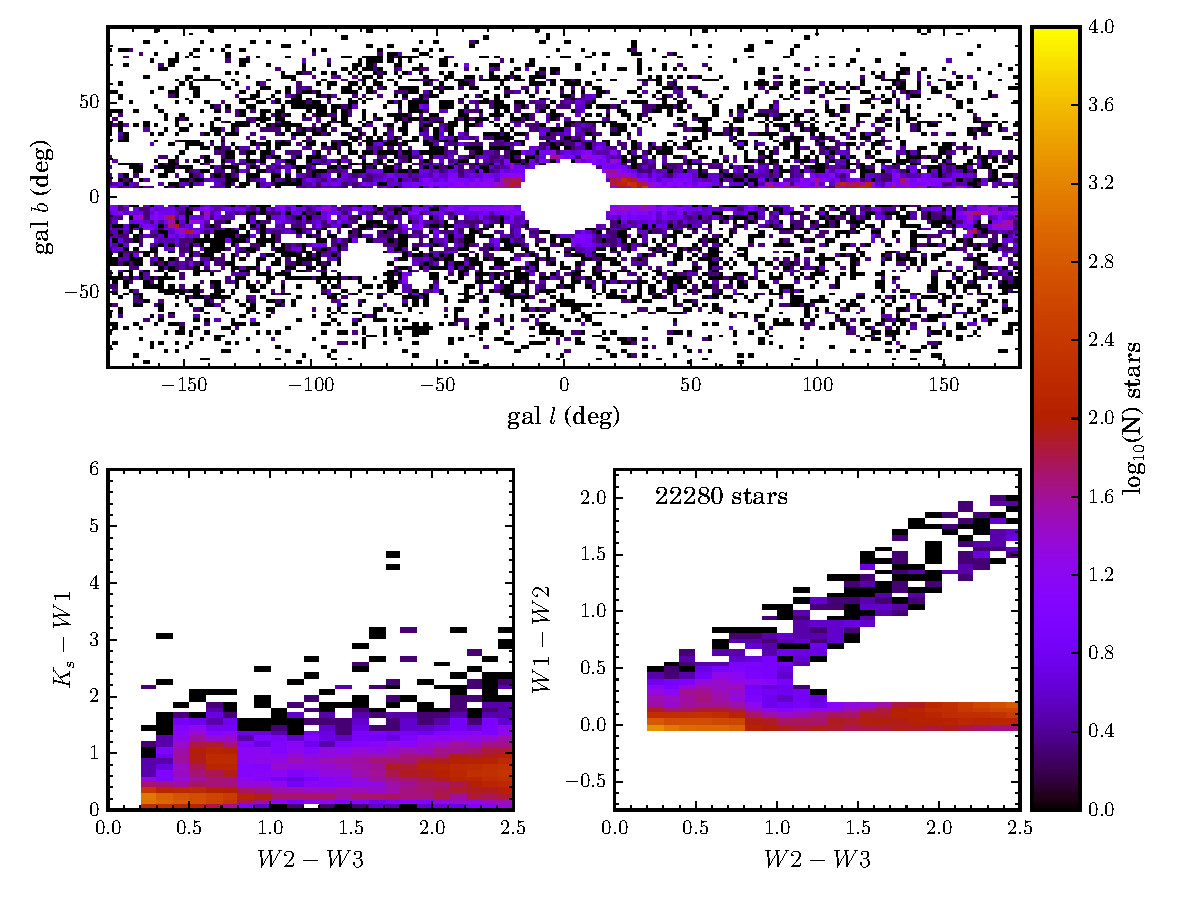
\includegraphics[width=6.5in]{figs/color_and_map_candidates_region0.pdf}
\caption{\label{fig:color_map_candidates0}}
\end{figure}

\begin{figure}[h]
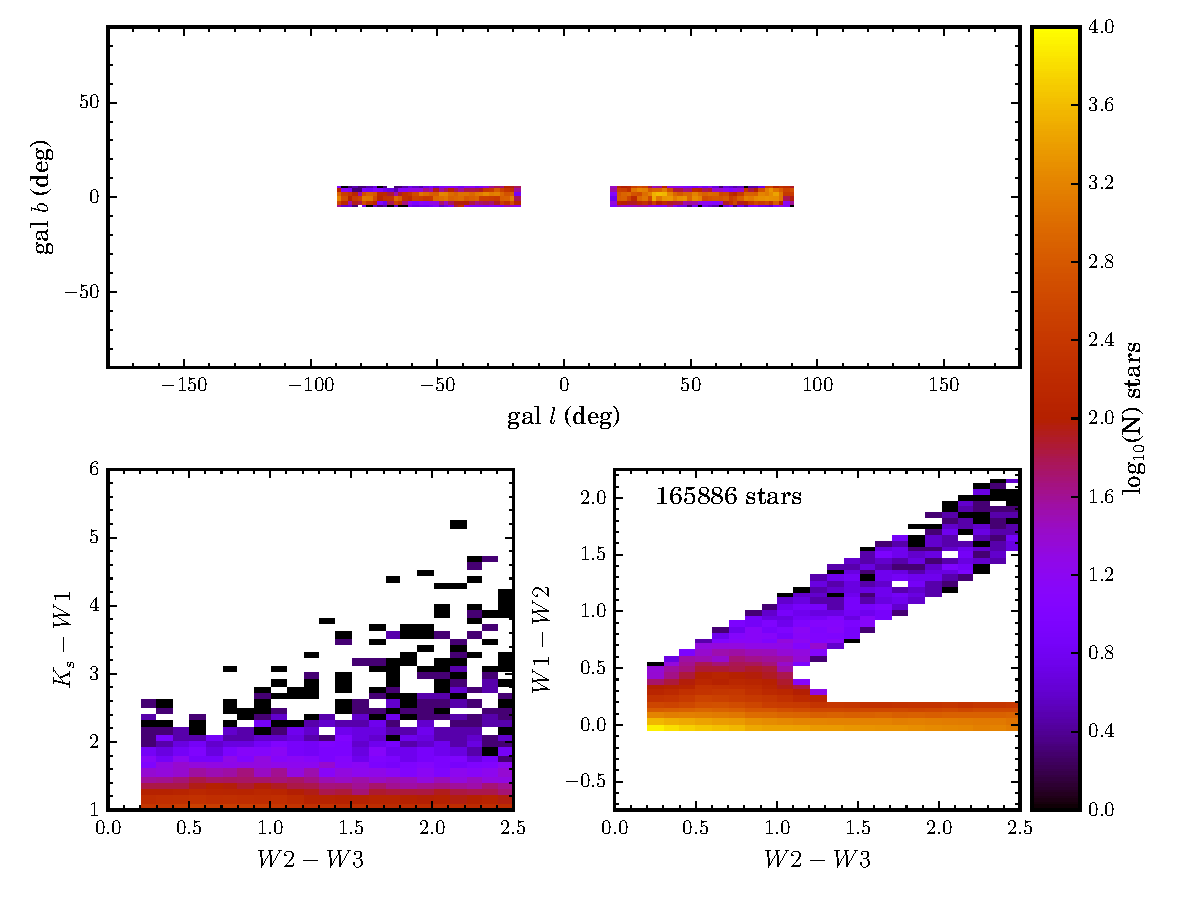
\includegraphics[width=6.5in]{figs/color_and_map_candidates_region1.pdf}
\caption{\label{fig:color_map_candidates1}}
\end{figure}

\begin{figure}[h]
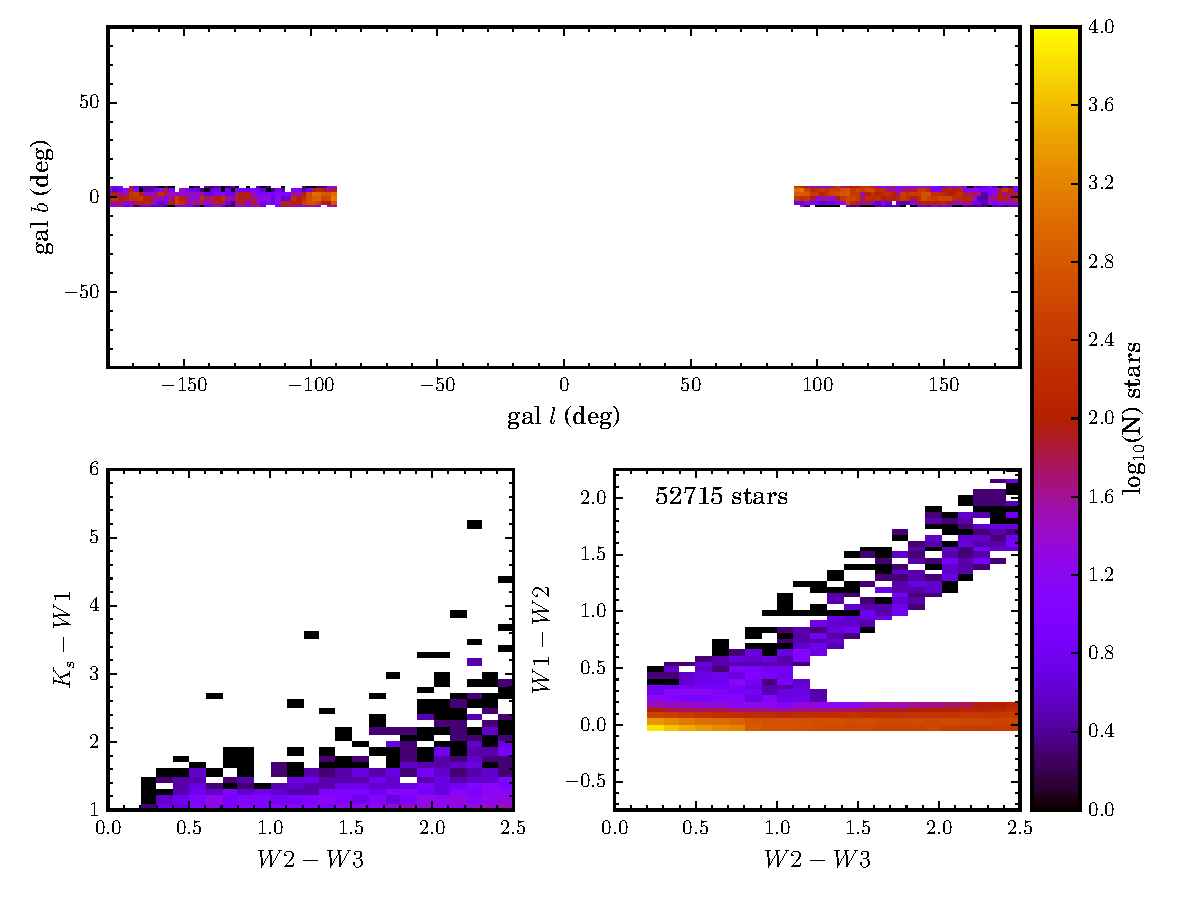
\includegraphics[width=6.5in]{figs/color_and_map_candidates_region2.pdf}
\caption{\label{fig:color_map_candidates2}}
\end{figure}

\begin{figure}[h]
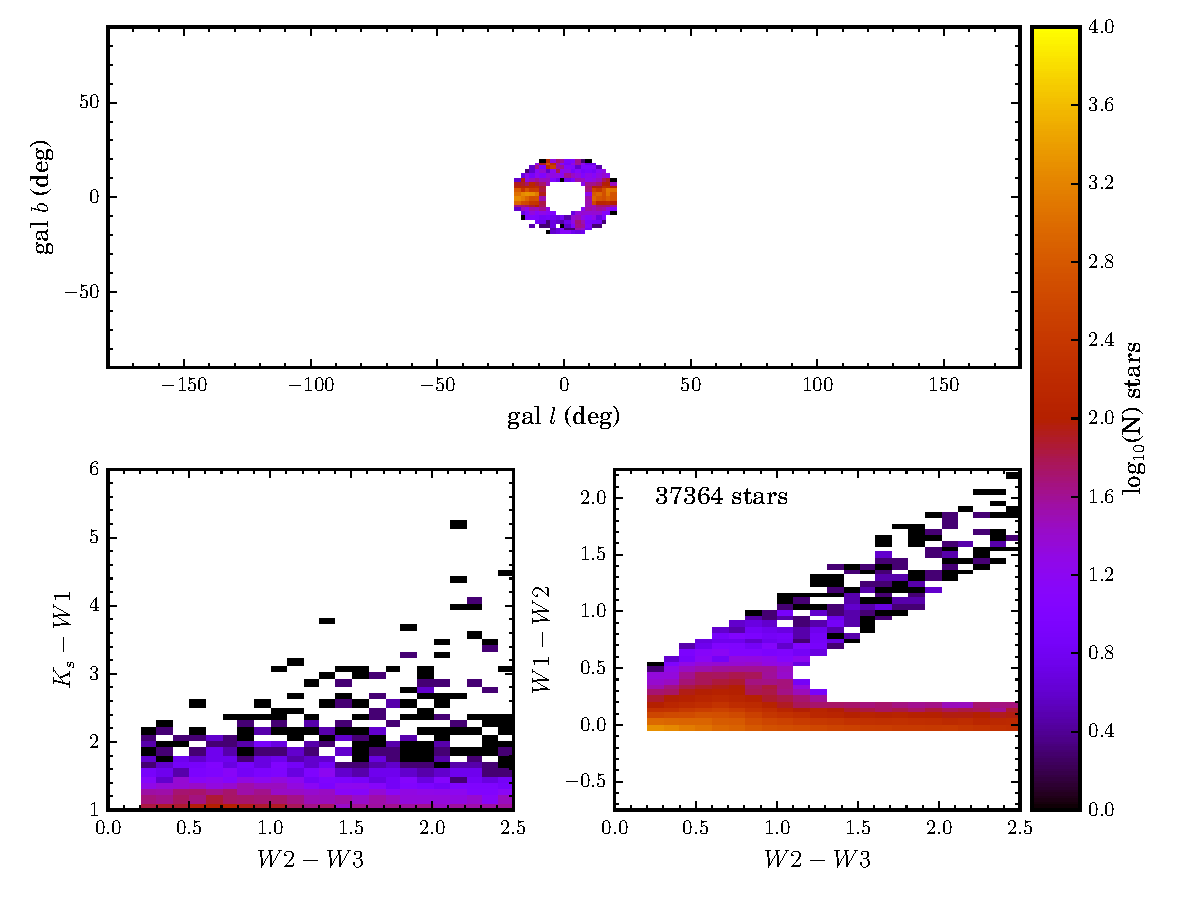
\includegraphics[width=6.5in]{figs/color_and_map_candidates_region3.pdf}
\caption{\label{fig:color_map_candidates3}}
\end{figure}

\begin{figure}[h]
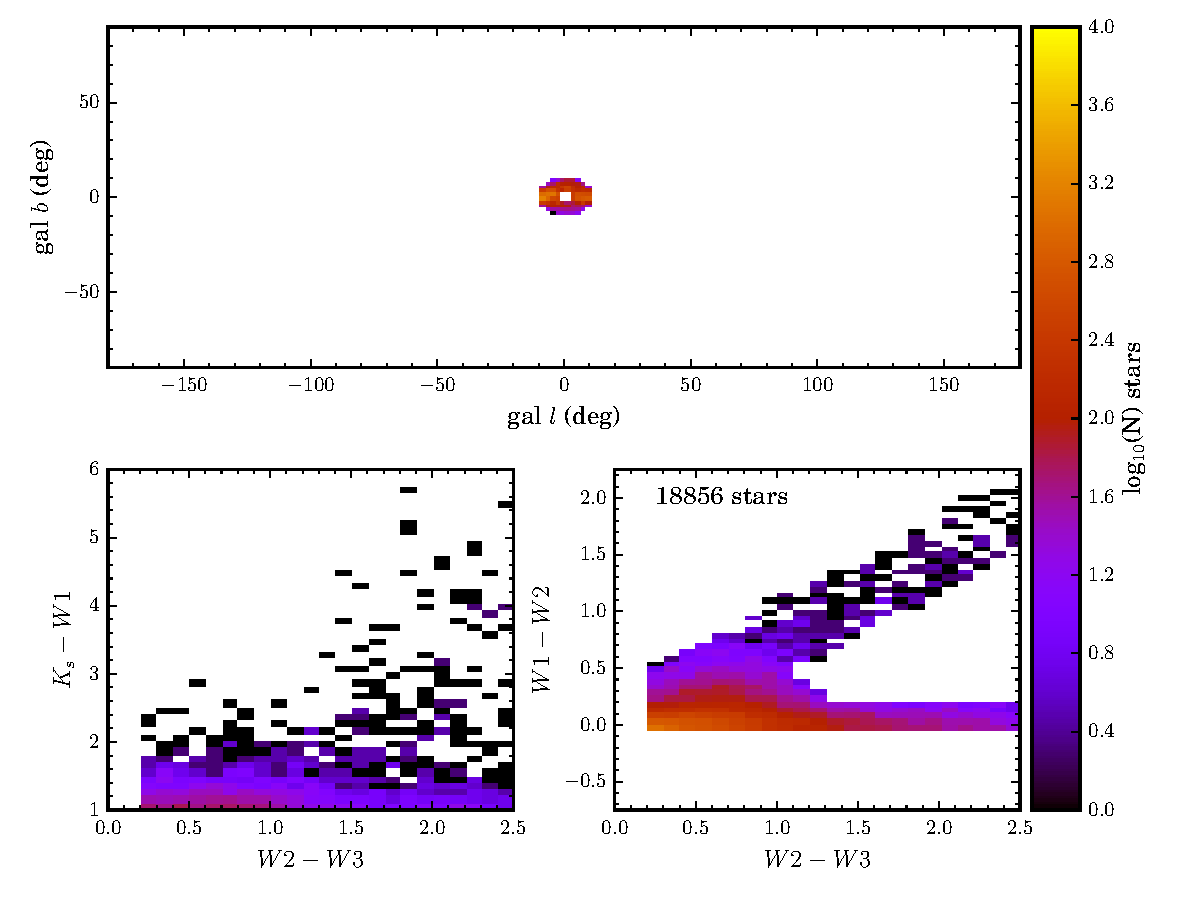
\includegraphics[width=6.5in]{figs/color_and_map_candidates_region4.pdf}
\caption{\label{fig:color_map_candidates4}}
\end{figure}

\begin{figure}[h]
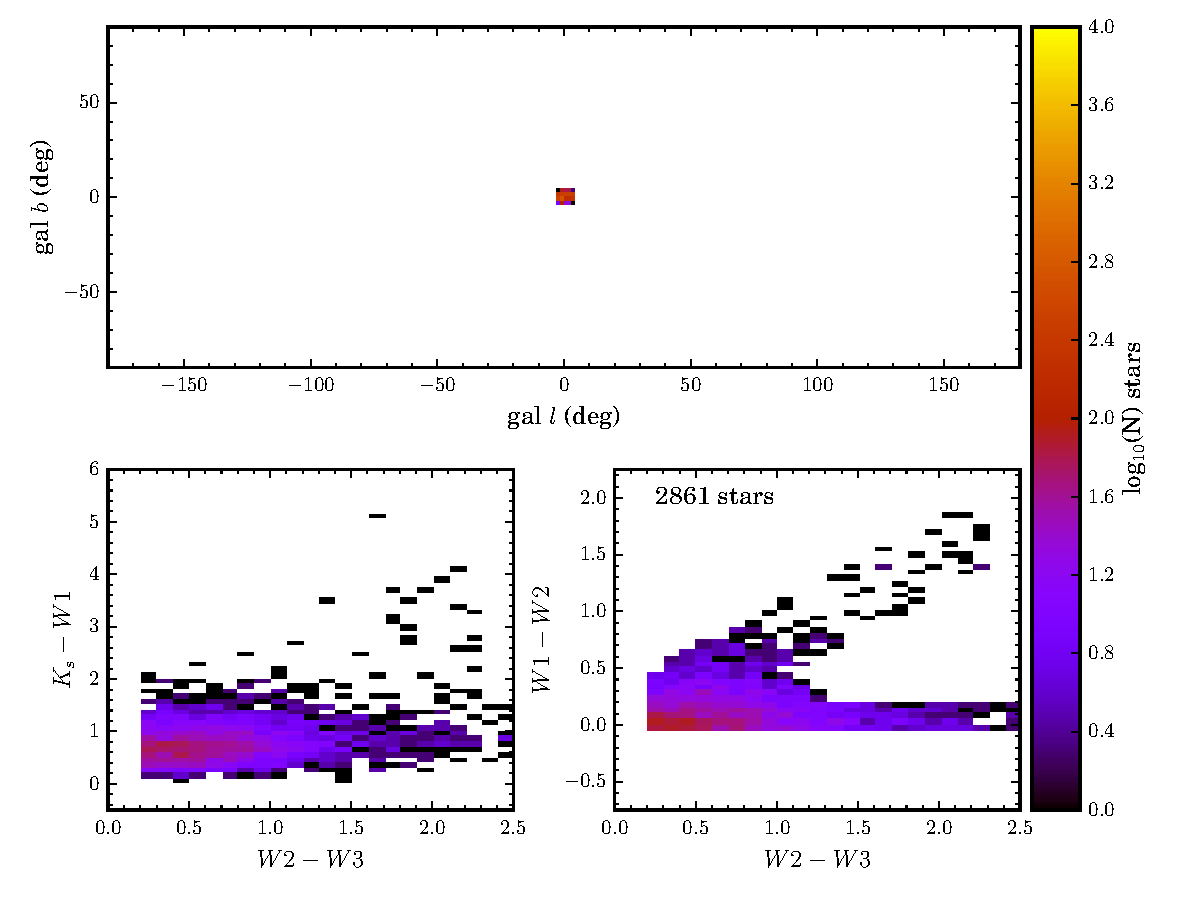
\includegraphics[width=6.5in]{figs/color_and_map_candidates_region5.pdf}
\caption{\label{fig:color_map_candidates5}}
\end{figure}


\subsection{O-rich and C-rich AGB Candidates}
%This section should be somewhat substantial, as you did a lot to get from the previous one through to the end of this one. You used the known AGB stars from OGLE matched to WISE in addition to some help from Nikutta et al 2014 to define O-rich and C-rich boundaries for AGB stars in color-color space. Talk about how these boundaries reduced your sample. Also talk about how these selections of stars were used to estimate  color-magnitude relationships for AGB stars with the LMC as reference, and find some way to justify the 2 magnitude offset that makes the results approach believability. Then talk about how distances were calculated. It was an iterative process that used a test distance to calculate the expected dust column along the line of sight until the sum of distance modulus and extinction coefficient matched apparent minus absolute magnitude. What were the steps in distance modulus? How did you get the extinction coefficient from the color excess that's actually output from galfastdust? What's the source for the galfastdust estimation procedure? And what are the results for the distance measurement?

\subsection{Galactic Number Density}
%This is the section where we show that what we've done is not complete bullshit, though some fecal flecks may remain. The big fig is going to be that plot of |Z| vs. R

% Conclusions
\section{Conclusions}
\label{sec:conclusions}
Put words here

% References
\bibliographystyle{apj}
\bibliography{thesisproprefs}
\end{document}
